
\documentclass[12pt]{article}
\usepackage[utf8]{inputenc}
\usepackage[T1]{fontenc}
\usepackage{amsmath}
\usepackage{amsfonts}
\usepackage{amssymb}
\usepackage{graphicx}
\usepackage{array}
\usepackage{multirow}
\usepackage{geometry}
\usepackage{float}
\usepackage{tabularray}
\usepackage{listings}
\usepackage{xcolor}

\geometry{legalpaper, margin=1.5cm}
\lstdefinestyle{sqlStyle}{
	language=SQL,
	basicstyle=\ttfamily\small,
	keywordstyle=\color{blue},
	stringstyle=\color{red},
	commentstyle=\color{green!50!black},
	showstringspaces=false,
	breaklines=true,
	breakatwhitespace=true,
	tabsize=4,
	numbers=left,
	numberstyle=\scriptsize\color{gray},
	frame=single,
	frameround=tttt,
	rulecolor=\color{black},
	backgroundcolor=\color{gray!10},
	captionpos=b
}


\begin{document}

	\begin{center}
		\Huge RAPORT
	\end{center}

	\begin{table}[h!]
		\centering
		\begin{tblr}{
				width = \linewidth,
				colspec = {Q[156]Q[156]Q[156]Q[156]Q[156]Q[156]},
				row{1} = {c},
				column{4} = {c},
				column{6} = {c},
				cell{1}{1} = {c=6}{0.936\linewidth},
				cell{2}{2} = {c=5}{0.803\linewidth},
				cell{3}{2} = {c=5}{0.803\linewidth},
				cell{4}{2} = {c},
				cell{5}{2} = {c=5}{0.803\linewidth},
				hline{1,6} = {1}{-}{leftpos = 1, rightpos = 1},
				hline{1,6} = {2}{-}{leftpos = 1, rightpos = 1},
				hline{2,2} = {1}{-}{leftpos = 1, rightpos = 1},
				hline{2,2} = {2}{-}{leftpos = 1, rightpos = 1},
				vline{1,1} = {1}{-}{abovepos = 1, belowpos = 1},
				vline{1,1} = {2}{-}{abovepos = 1, belowpos = 1},
				vline{7,1} = {1}{-}{abovepos = 1, belowpos = 1},
				vline{7,1} = {2}{-}{abovepos = 1, belowpos = 1},
				hlines,
				vlines,
			}
			{AKADEMIA NAUK STOSOWANYCH W NOWYM SĄCZU\\Wydział Nauk Inżynieryjnych, Katedra informatyki} &  &  &  &  &  \\
			Przedmiot:  & Bazy danych          &  &  &  &  \\
			Temat:      & Aplikacja z bazą danych MySql - Lista zakupów - "Shopping dashboard"                       &  &  &  &  \\
			Grupa:      & IS-2(s)P2 & Data: & 24.05.2023 \\
			Osoby:      & Justyna Jachowicz
			&  &  &  &
		\end{tblr}
	\end{table}


	\section{Wykonane zadania}
	\begin{enumerate}
		\item Dodanie nowego repozytorium aplikacji Java
		\item Implementacja logiki - połączenie bazy danych z kodem Java
		\item Dodanie skryptu SQL dodającego produkty podczas startu aplikacji
		\begin{lstlisting}[style=sqlStyle, caption=data.sql, label=lst:sqlCode]
			INSERT INTO shopping_dashboard.product (brand, price, product_name, weight,  quantity) VALUES('Bielmar',6.2, 'Margaryna palma', 0.4, 120);
			INSERT INTO shopping_dashboard.product (brand, price, product_name, weight,  quantity) VALUES('Cola Co',8.6, 'Coca Cola', 1, 1500);
			INSERT INTO shopping_dashboard.product (brand, price, product_name, weight,  quantity) VALUES('Piekarnia Grzes',4.5, 'Chleb', 0.6, 80);
			INSERT INTO shopping_dashboard.product (brand, price, product_name, weight,  quantity) VALUES('Nestle',2.8, 'Snickers', 0.4, 120);
			INSERT INTO shopping_dashboard.product (brand, price, product_name, weight,  quantity) VALUES('Kryniczanka',2.2, 'Woda mineralna gazowana', 1.5, 300);
			INSERT INTO shopping_dashboard.product (brand, price, product_name, weight,  quantity) VALUES('Nestle',6.2, 'Platki sniadaniowe', 5.5, 120);
		\end{lstlisting}
		\item Wykonanie schematu bazy danych
		\begin{figure}[H]
			\centering
			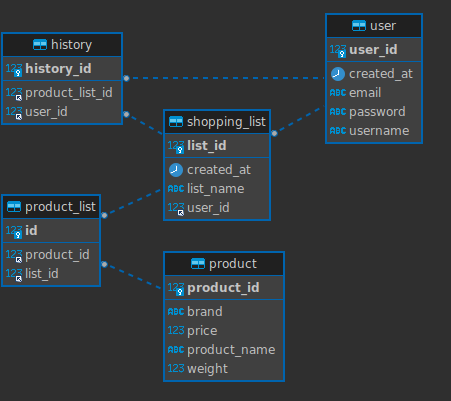
\includegraphics{schemat_mysql}
			\label{fig:schematmysql}
		\end{figure}

		\item Dodanie widoku do wyświetlania danych
		\begin{figure} [H]
			\centering
			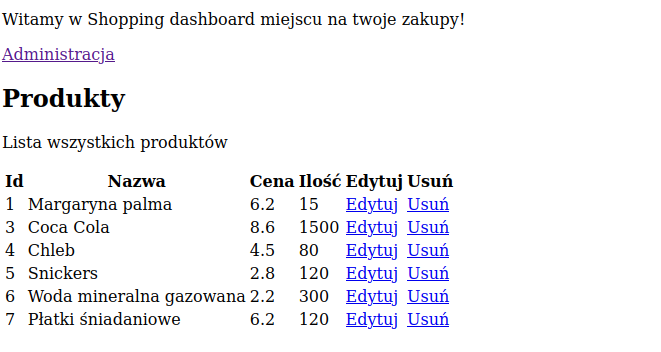
\includegraphics{widok}
			\label{fig:widok}
		\end{figure}
	\end{enumerate}
	\section{Poświęcony czas}
	\begin{itemize}
		\item 8 godzin
	\end{itemize}
	\section{Zadania na kolejny tydzień}
	\begin{enumerate}
		\item Dodanie możliwości edytowania, usuwania i dodawania produktów
		\item Dodanie możliwości utworzenia listy per użytkownik
	\end{enumerate}
	\section{Przypadek użycia}
	\begin{enumerate}
	\item Klient przed zakupami robi listę produktów
	\item Po zakupach klietnt zaznacza co kupił, w jakim sklepie, i za jaką kwotę
	\item Po dokonaniu wielu zakupów po jakimś czasie klient ma  możliwości sprawdzenia średniej ceny danego produktu, oraz gdzie najczęsicej kupuje, i gdzie się najbardziej opłaca
	\end{enumerate}
\end{document}